\documentclass{beamer}


\mode<presentation>
{
  \usetheme{CambridgeUS}
	\usecolortheme{beaver}
  % or ...

  \setbeamercovered{transparent}
  % or whatever (possibly just delete it)
}


\usepackage{xeCJK}
\usepackage{ulem}
\usepackage[english]{babel}
\usepackage[utf8]{inputenc}
\usepackage{times}
\usepackage[T1]{fontenc}
\usepackage{hyperref}
\usepackage{pifont}
\usepackage{biblatex}
\usepackage{bibentry}
\usepackage{verbatim}
\usepackage[absolute,overlay]{textpos}
\bibliography{cite}
\newcommand{\cmark}{\ding{51}}%
\newcommand{\xmark}{\ding{55}}%
\setCJKmainfont{WenQuanYi Micro Hei}
\renewcommand{\raggedright}{\leftskip=0pt \rightskip=0pt plus 0cm}
\raggedright

\let\oldfootnotesize\footnotesize
\renewcommand*{\footnotesize}{\oldfootnotesize\tiny}

\title[Intelligent Software Engineering] 
{Intelligent Software Engineering}
\subtitle{Software Testing}

\author[Zhilei Ren] 
{Zhilei Ren}

\institute[Dalian University of Technology] % (optional, but mostly needed)
{
\\
\includegraphics[width=0.1\textwidth]{../utils/logo.png}\\
Dalian University of Technology
}


\subject{Software Engineering}



\pgfdeclareimage[width=0.08\textwidth]{university-logo}{../utils/logo.png}
\logo{\pgfuseimage{university-logo}}



% Delete this, if you do not want the table of contents to pop up at
% the beginning of each subsection:

\AtBeginSection[]
{
  \begin{frame}<beamer>{Outline}
    \tableofcontents[currentsection,currentsubsection]
  \end{frame}
}
\AtBeginSubsection[]
{
  \begin{frame}<beamer>{Outline}
    \tableofcontents[currentsection,currentsubsection]
  \end{frame}
}


% If you wish to uncover everything in a step-wise fashion, uncomment
% the following command: 

%\beamerdefaultoverlayspecification{<+->}

\setbeamertemplate{section in toc}[circle]
\setbeamertemplate{items}[circle]
\setbeamertemplate{caption}[numbered]
\setbeamertemplate{bibliography item}{\insertbiblabel}
\setbeamertemplate{bibliography entry title}{}
\setbeamertemplate{bibliography entry journal}{}

\begin{document}

\begin{frame}
  \titlepage
\end{frame}

%\begin{frame}{Outline}
%  \tableofcontents[currentsection,currentsubsection, 
%    hideothersubsections, 
%    sectionstyle=show,
%]
%\end{frame}

\begin{frame}{Outline}
  \tableofcontents[currentsection,currentsubsection, 
    sectionstyle=show,
    subsectionstyle=show,
]
\end{frame}

\AtBeginSubsection[]
{
  \begin{frame}<beamer>{Outline}
    \tableofcontents[currentsection,currentsubsection]
  \end{frame}
}

\section{The Eternal Battle: Bugs, Debugging, and Testing}

\begin{frame}[t]{1947: The First "Computer Bug"}
\begin{columns}
    \begin{column}{0.5\textwidth}
        \begin{itemize}
            \item \textbf{September 9, 1947}: Operators of the Harvard Mark II computer found a moth trapped in a relay.
            \item The term "bug" had been used in engineering before, but this incident popularized it in computing.
            \item The moth was taped into the logbook with the note: "First actual case of bug being found."
            \item \textbf{Debugging} literally started as removing insects from hardware.
        \end{itemize}
    \end{column}
    \begin{column}{0.5\textwidth}
        \begin{figure}
        \begin{center}
            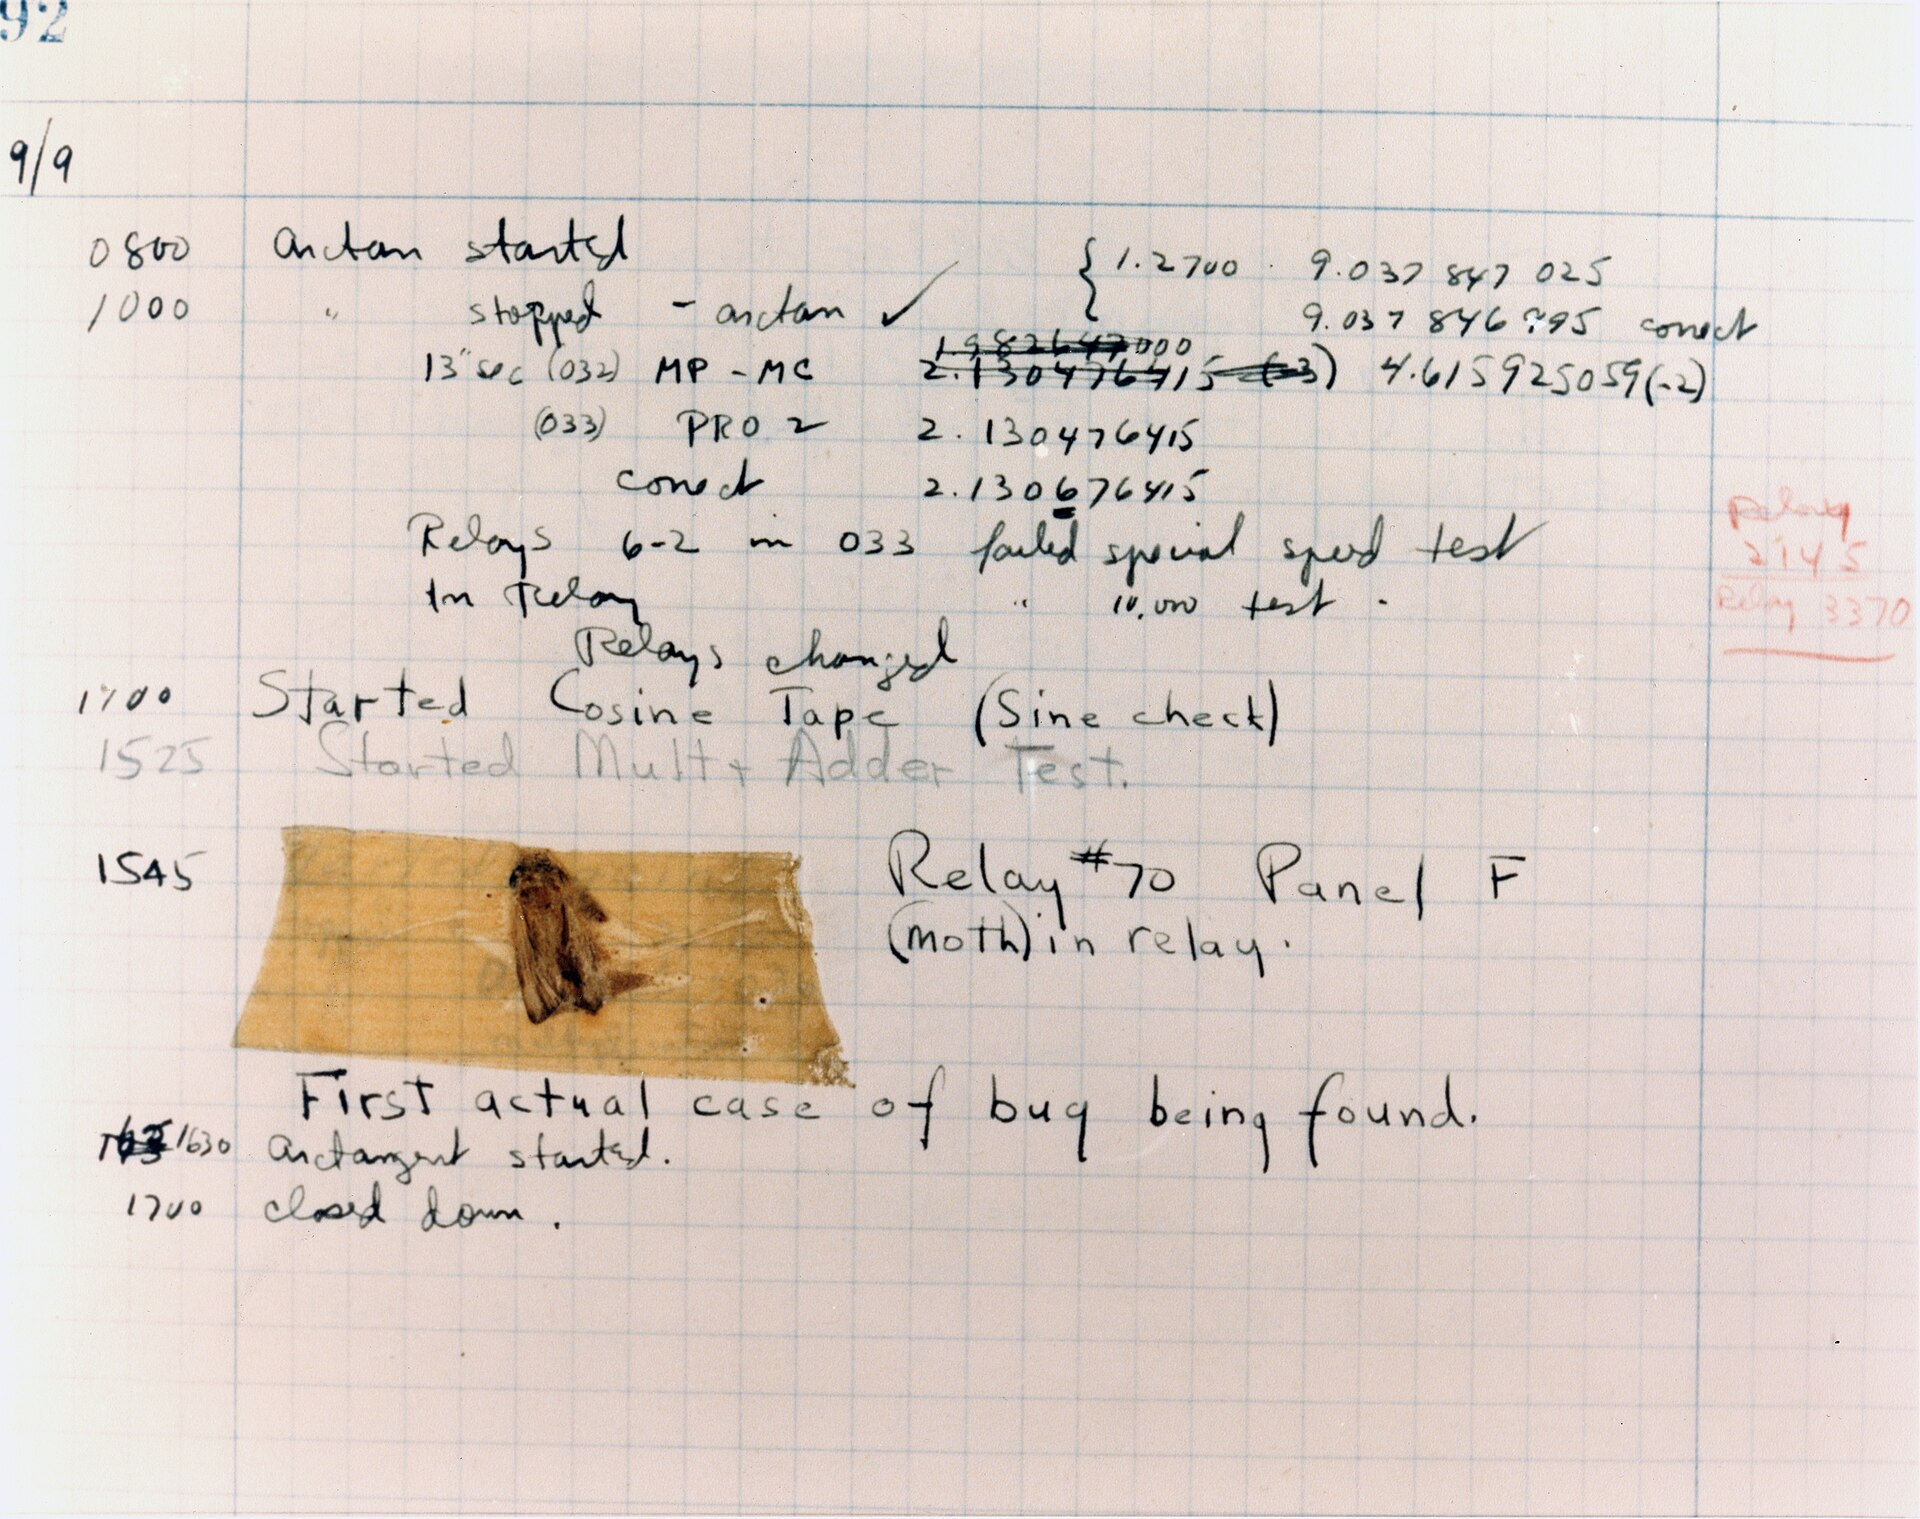
\includegraphics[width=0.9\textwidth]{images/first-computer-bug.jpg}
        \end{center}
        \caption{The first computer "bug" from the Harvard Mark II log book.}
        \label{fig:bug}
        \end{figure}
        
    \end{column}
\end{columns}
\begin{block}{}
Early "debugging" was a physical, hardware-centric activity.
\end{block}
\end{frame}

\begin{frame}[t]{1950s-1960s: The Dawn of Software Debugging}
\begin{itemize}
    \item \textbf{Print Statement Debugging}: The simplest and most enduring method. Programmers inserted print statements to trace program execution and variable states.
    \item \textbf{Core Dumps}: Analyzing the contents of memory after a program crash. A low-level, complex, but powerful technique.
    \item \textbf{Ad-hoc Testing}: Testing was manual, informal, and often performed by the developers themselves near the end of the project.
    \item \textbf{The Challenge}: As software grew in complexity, these methods became insufficient. The "software crisis" was, in part, a crisis of quality and reliability.
\end{itemize}
\begin{center}
    \texttt{printf("Got here! Value of x = \%d \textbackslash n", x);} % Example of a print statement
\end{center}
\end{frame}

\begin{frame}[t]{1970s-1980s: Formalizing Testing and Tools}
\begin{columns}
    \begin{column}{0.6\textwidth}
        \textbf{The Rise of Testing Theory}
        \begin{itemize}
            \item \textbf{Black-box vs. White-box Testing}: Distinguishing between testing functionality (black-box) and testing internal structures (white-box).
            \item \textbf{Levels of Testing}: Unit, Integration, System, and Acceptance testing became standard concepts.
            \item \textbf{Static Analysis}: Compilers began to include more sophisticated warnings for potential code issues.
        \end{itemize}
        \textbf{The First Debugging Tools}
        \begin{itemize}
            \item \textbf{Symbolic Debuggers} (e.g., gdb): Allowed programmers to interact with a running program, set breakpoints, and inspect variables symbolically.
            \item This was a monumental leap from raw core dumps.
        \end{itemize}
    \end{column}
    \begin{column}{0.4\textwidth}
        % \includegraphics[width=0.8\textwidth]{images/gdb-screenshot.png}
        \\\scriptsize{Early GNU Debugger (GDB) interface.}
    \end{column}
\end{columns}
\end{frame}

\begin{frame}[t]{1990s: Automation and Process Integration}
\begin{itemize}
    \item \textbf{Automated Regression Testing}: Tools like JUnit (1997) for Java, created by Kent Beck and Erich Gamma, revolutionized testing.
    \begin{itemize}
        \item Tests could be run automatically and frequently.
        \item Provided a safety net for refactoring and adding new features.
        \item Embodied the \textbf{Test-Driven Development (TDD)} philosophy.
    \end{itemize}
    \item \textbf{Testing Becomes a Discipline}: The role of \textbf{Quality Assurance (QA) Engineer} became specialized.
    \item \textbf{Continuous Integration (CI)}: Tools like CruiseControl automated the process of building and testing software after every change, catching integration bugs early.
\end{itemize}
\begin{center}
    % \includegraphics[width=0.7\textwidth]{images/junit-logo.png}
\end{center}
\end{frame}

\begin{frame}[t]{2000s-2010s: Scaling and Shifting Quality Left}
\begin{columns}
    \begin{column}{0.45\textwidth}
        \textbf{Paradigm Shifts}
        \scriptsize
        \begin{itemize}
            \item \textbf{Shift-Left Testing}: The idea of testing earlier in the development lifecycle, involving QA and writing tests during development, not after.
            \item \textbf{Test Automation Pyramid}: A strategy for a balanced test suite: many fast, cheap Unit tests; fewer Integration tests; even fewer UI tests.
            \item \textbf{DevOps and Quality}: With rapid deployments, automated testing became non-negotiable. Quality is everyone's responsibility.
        \end{itemize}
        \normalsize
        \textbf{New Frontiers}
        \scriptsize
        \begin{itemize}
            \item \textbf{Selenium}: Automated web browser testing.
            \item \textbf{Chaos Engineering}: Deliberately injecting failures into systems (e.g., Netflix's Chaos Monkey) to build resilience.
        \end{itemize}
    \end{column}
    \begin{column}{0.45\textwidth}
        \begin{figure}
        \begin{center}
            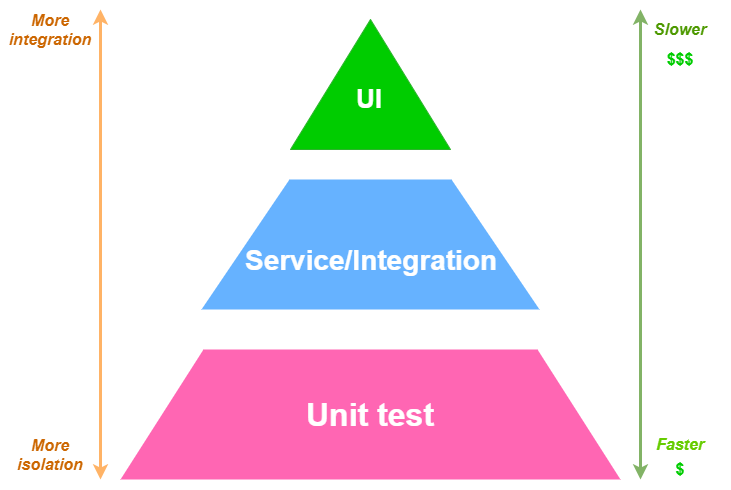
\includegraphics[width=\textwidth]{images/test-pyramid.png}
        \end{center}
        \caption{Test Automation Pyramid}
        \label{fig:}
        \end{figure}
        
    \end{column}
\end{columns}
\end{frame}

\begin{frame}[t]{2020s: The AI-Powered Future of Debugging}
\begin{itemize}
    \item \textbf{AI-Assisted Testing}:
    \begin{itemize}
        \item AI generates test cases, predicts flaky tests, and optimizes test suites.
        \item Tools can automatically detect visual regressions in UI.
    \end{itemize}
    \item \textbf{Intelligent Fault Localization}:
    \begin{itemize}
        \item AI analyzes code, execution traces, and bug reports to suggest the most likely lines of code causing a failure.
        \item \textbf{Example}: A tool like \textbf{Amazon CodeGuru} or \textbf{OpenAI's Debugger} can point directly to the suspicious code.
    \end{itemize}
    \item \textbf{Automated Program Repair}:
    \begin{itemize}
        \item LLMs can not only find bugs but also suggest and even generate fixes.
        \item \textbf{Example}: GitHub Copilot Chat can explain a bug and propose a patch.
    \end{itemize}
    \item \textbf{Observability}: The evolution beyond monitoring. Using logs, metrics, and traces (the three pillars) to understand the internal state of a system by its external outputs, making debugging in production much more effective.
\end{itemize}
\end{frame}

\begin{frame}[t]{The Evolution of Debugging at a Glance}
\begin{center}
    \scriptsize
    \begin{tabular}{|l|l|l|}
    \hline
    \textbf{Era} & \textbf{Primary Method} & \textbf{Testing Focus} \\
    \hline
    1940s-50s   & Physical Inspection & Ad-hoc \\
    \hline
    1960s-70s   & Print Statements & Manual, Late \\
    \hline
    1980s-90s   & Interactive Debuggers  & Formalized Test Levels \\
    \hline
    2000s-10s   & CI/CD Integrated Tools & Shift-Left, Automation \\
    \hline
    2020s+      & AI-Powered Analysis & AI-Generated Tests \\
    \hline
    \end{tabular}
\end{center}
\vspace{1em}
\begin{block}{The Unchanging Goal}
To move from \alert{reactive} bug-fixing to \alert{proactive} bug-prevention, and to reduce the time between discovering a failure and fixing it from months to minutes.
\end{block}
\end{frame}

\section{Taxonomy of Software Testing}
\label{sec:concept}
\begin{frame}[t]{Software Testing}

    Software testing is the process of evaluating and verifying that a software product or application functions correctly, securely and efficiently according to its specific requirements\footnote{\url{https://www.ibm.com/think/topics/software-testing}}.
\end{frame}

\begin{frame}[t]{Testing Phases}
    \begin{block}
        {Unit Testing}
Unit testing tests the individual components of software with the purpose of verifying the correctness of the basic units of software design. The object of testing is the smallest unit of software design: functions.
    \end{block}
\end{frame}

\begin{frame}[t]{Testing Phases}
    \begin{block}{Integration Testing}
Integration testing, also known as comprehensive testing, assembly testing, or joint testing, involves assembling program modules using appropriate integration strategies and testing the interfaces and integrated functionality. Its main purpose is to check whether the interfaces between software units are correct. The objects of integration testing are modules that have already undergone unit testing.
    \end{block}
\end{frame}

\begin{frame}[t]{Testing Phases}
    \begin{block}{System Testing}
System testing mainly includes functional testing, interface testing, reliability testing, usability testing, and performance testing. Functional testing primarily focuses on aspects such as functional availability, degree of functional implementation (functional processes \& business processes, data processing \& business data processing).
    \end{block}
\end{frame}

\begin{frame}[t]{Testing Phases}
    \begin{block}{Regression Testing}
Regression testing refers to testing activities conducted during the software maintenance phase to detect errors introduced by code modifications. Regression testing is an important task in the software maintenance phase, with studies showing that the cost of regression testing accounts for more than one-third of the total cost of the software lifecycle.

Unlike ordinary testing, at the beginning of the regression testing process, testers have a complete set of test cases available. Therefore, how to effectively reuse existing test case sets based on code modifications is an important direction in regression testing research. Additionally, research directions in regression testing involve automation tools, object-oriented regression testing, test case prioritization, and supplementary generation of regression test cases.
\end{block}
\end{frame}

\begin{frame}[t]{Unit Testing}
In computer programming, unit testing (English: Unit Testing), also known as module testing, is testing work conducted to verify the correctness of program modules (the smallest units of software design). A program unit is the smallest testable component of an application. In procedural programming, a unit is a single program, function, procedure, etc.; for object-oriented programming, the smallest unit is a method, including methods in base classes (superclasses), abstract classes, or derived classes (subclasses).

Each ideal test case is independent of other cases; to isolate modules during testing, test harness programs such as stubs, mocks, or fakes are often used. Unit testing is typically written by software developers to ensure that their code meets software requirements and follows development goals. Its implementation can be very manual or integrated as part of build automation.\footnote{\url{https://en.wikipedia.org/wiki/Unit_testing}}
\end{frame}

\begin{frame}[t]{Test Oracle}
A test oracle, also known as a test criterion, is a mechanism used by software testers or software engineers to determine whether a test has passed. The test oracle determines the expected output of the product for a given test case input, which is then compared with the output of the system under test.

Common test oracles include:

\begin{itemize}
    \item Design specifications and software documentation
    \item Other products (for example, as a test oracle for a software program, it might be another program that computes the same mathematical expression using a different algorithm)
    \item "Heuristic oracles" that provide approximate or accurate results for a small set of test inputs
    \item "Statistical oracles" that use statistical features
    \item "Model-based oracles" that use the same model to generate and verify system behavior
\end{itemize}
\end{frame}

\begin{frame}[t]{Test Oracle}
    \centering
    \begin{columns}
        \begin{column}{0.3\textwidth}
            
            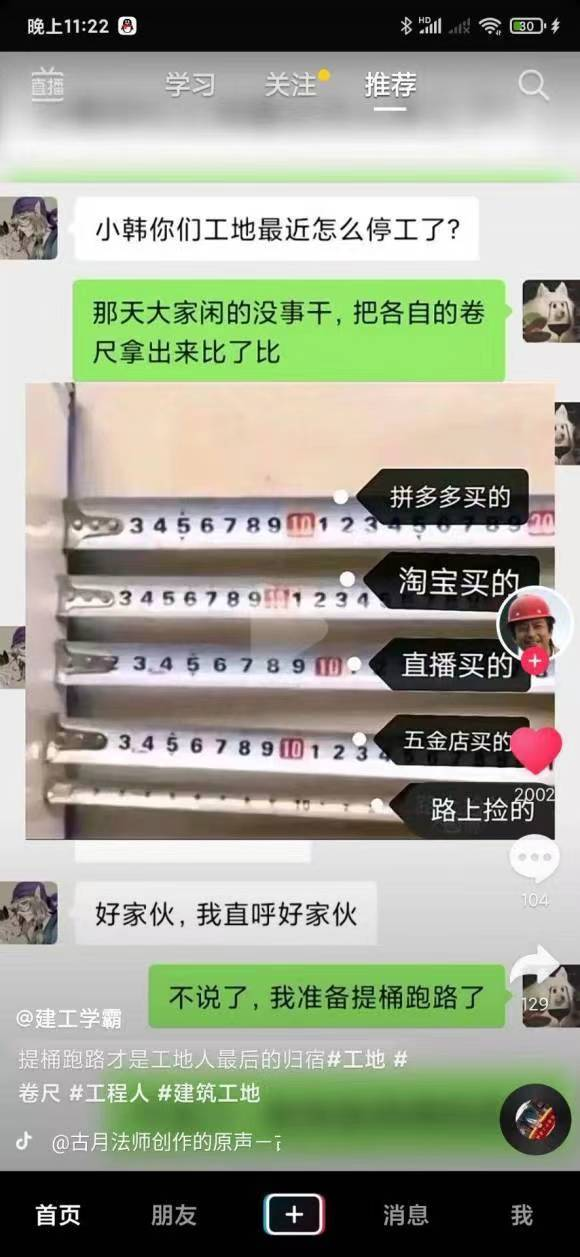
\includegraphics[width=0.9\linewidth]{images/differential.jpeg} % Replaced with example-image as requested
        \end{column}
        \begin{column}{0.5\textwidth}
            \scriptsize
            \begin{itemize}
                \item A: ``Hey Han, how come your construction site shut down recently?''
                \item B: ``That day we had nothing to do, so we all took out our tape measures and compared them.''
                \item One bought from Temu.
                \item One from Taobao.
                \item One from a livestream sale.
                \item One from the hardware store.
                \item One picked up off the street.
                \item A: ``Holy moly, what a mess''.
                \item B: ``Anyway, I'm done talking. I'm gonna grab my bucket and run (quitting)''. 
            \end{itemize}
        \end{column}
    \end{columns}
    \begin{textblock}{4}(6,4)
        \only<2>{
            
\includegraphics[width=\textwidth]{images/bucket-run.jpeg}
        }
    \end{textblock}
\end{frame}

\begin{frame}[t]{Fun Fact}
	\begin{block}
		{Xfce Bug \#12117}The defualt wallpaper is having my animal scritch all the plastic off my LED MONITOR! Can we choose a different wallpaper? I cannot expect the scratches and whu not? Let's end the mouse games over here.\footnote{\url{https://bugzilla.xfce.org/show_bug.cgi?id=12117}}
		
	\end{block}
	
\end{frame}
\begin{frame}[t]{Fun Fact}
	\centering
	
\includegraphics[width=0.5\linewidth]{images/cat-xfce-bug-2.jpg}
	
\end{frame}
\begin{frame}[t]{Fun Fact}
	
\includegraphics[width=0.8\linewidth]{images/patched-wallpaper.jpg}
	
\end{frame}
% section 基本概念 (end)
\section{Specialized Testing Types}

\begin{frame}[t]{Regression and Smoke Testing}
\begin{block}{Regression Testing}
\begin{itemize}
\item Ensures \textbf{new changes don't break} existing functionality
\item Critical during maintenance and enhancements
\item Often automated for efficiency
\end{itemize}
\end{block}

\begin{block}{Smoke Testing}
\begin{itemize}
\item \textbf{Basic functionality check} after build
\item Determines if further testing is feasible
\item "Build verification testing"
\end{itemize}
\end{block}
\end{frame}

\begin{frame}[t]{Exploratory and Negative Testing}
\begin{columns}[T]
\begin{column}{0.48\textwidth}
\textbf{Exploratory Testing}
\begin{itemize}
\item \textbf{Simultaneous learning and testing}
\item Relies on tester's creativity
\item Unscripted approach
\end{itemize}
\end{column}
\begin{column}{0.48\textwidth}
\textbf{Negative Testing}
\begin{itemize}
\item Validates system with \textbf{invalid inputs}
\item Checks \textbf{error handling}
\item Ensures system robustness
\end{itemize}
\end{column}
\end{columns}
\end{frame}

\section{Test-Driven Software Development}

\begin{frame}[t]{Test-Driven Development\footnote{\url{https://en.wikipedia.org/wiki/Test-driven_development}}}
    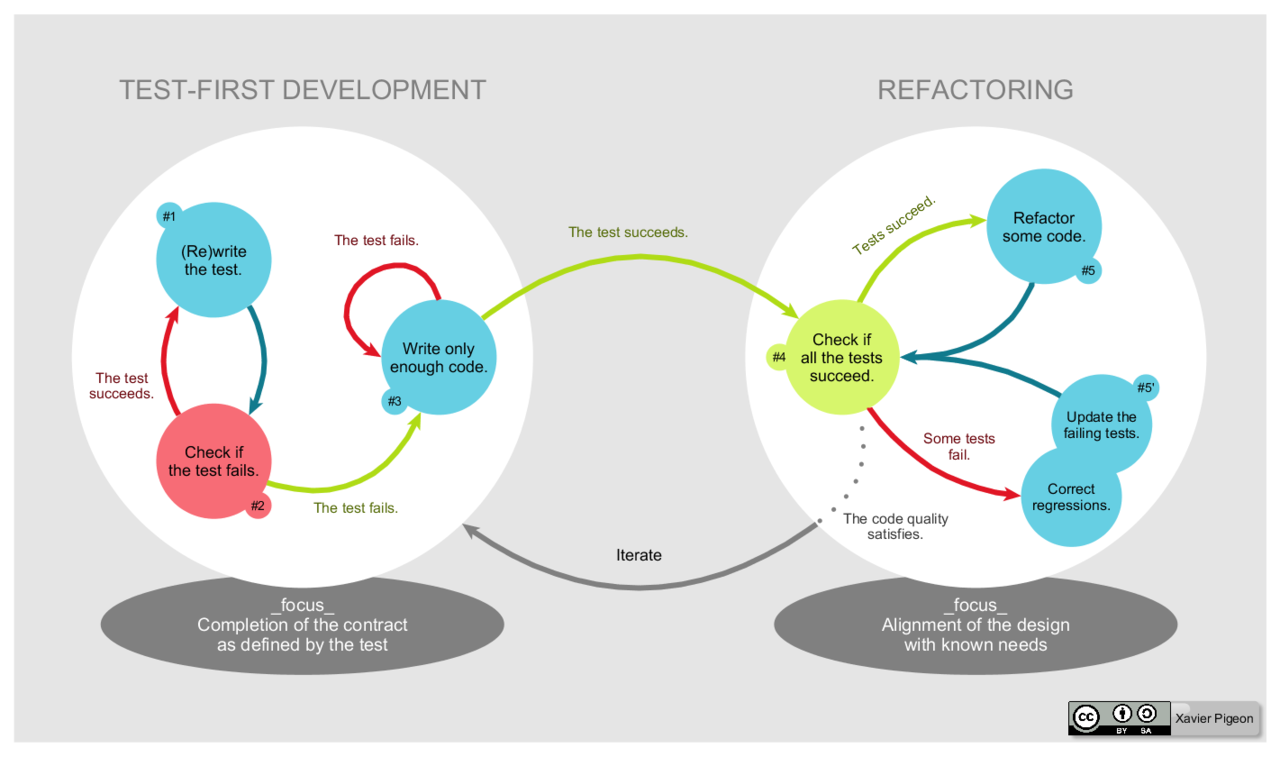
\includegraphics[width=0.8\linewidth]{images/TDD-Global-Lifecycle.png}
    
\end{frame}

\begin{frame}[t]{Add a test}
In test-driven development, each new feature begins with writing a test. Write a test that defines a function or improvements of a function, which should be very succinct. To write a test, the developer must clearly understand the feature's specification and requirements. The developer can accomplish this through use cases and user stories to cover the requirements and exception conditions, and can write the test in whatever testing framework is appropriate to the software environment. It could be a modified version of an existing test. This is a differentiating feature of test-driven development versus writing unit tests after the code is written: it makes the developer focus on the requirements before writing the code, a subtle but important difference.
    
\end{frame}


\begin{frame}[t]{Run all tests and see if the new test fails}
This validates that the test harness is working correctly, shows that the new test does not pass without requiring new code because the required behavior already exists, and it rules out the possibility that the new test is flawed and will always pass. The new test should fail for the expected reason. This step increases the developer's confidence in the new test.
    
\end{frame}

\begin{frame}[t]{Write the code}
The next step is to write some code that causes the test to pass. The new code written at this stage is not perfect and may, for example, pass the test in an inelegant way. That is acceptable because it will be improved and honed in Step 5.
    
At this point, the only purpose of the written code is to pass the test. The programmer must not write code that is beyond the functionality that the test checks.
\end{frame}


\begin{frame}[t]{Run tests}
If all test cases now pass, the programmer can be confident that the new code meets the test requirements, and does not break or degrade any existing features. If they do not, the new code must be adjusted until they do.
    
\end{frame}


\begin{frame}[t]{Refactor code}
The growing code base must be cleaned up regularly during test-driven development. New code can be moved from where it was convenient for passing a test to where it more logically belongs. Duplication must be removed. Object, class, module, variable and method names should clearly represent their current purpose and use, as extra functionality is added. As features are added, method bodies can get longer and other objects larger. They benefit from being split and their parts carefully named to improve readability and maintainability, which will be increasingly valuable later in the software lifecycle. 
    
\end{frame}


\begin{frame}[t]{Repeat}
    
Starting with another new test, the cycle is then repeated to push forward the functionality. The size of the steps should always be small, with as few as 1 to 10 edits between each test run. If new code does not rapidly satisfy a new test, or other tests fail unexpectedly, the programmer should undo or revert in preference to excessive debugging. Continuous integration helps by providing revertible checkpoints. When using external libraries it is important not to make increments that are so small as to be effectively merely testing the library itself,[4] unless there is some reason to believe that the library is buggy or is not sufficiently feature-complete to serve all the needs of the software under development.
\end{frame}

\section{Research Topics in Software Testing}
\begin{frame}[t]{Fuzz Testing}
In programming and software development, fuzzing or fuzz testing is an automated software testing technique that involves providing invalid, unexpected, or random data as inputs to a computer program. The program is then monitored for exceptions such as crashes, failing built-in code assertions, or potential memory leaks\footnote{\url{https://en.wikipedia.org/wiki/Fuzzing}}.
\end{frame}

\begin{frame}[t]{Differential Testing}
Differential testing, also known as differential fuzzing, is a software testing technique that detect bugs, by providing the same input to a series of similar applications (or to different implementations of the same application), and observing differences in their execution. Differential testing complements traditional software testing because it is well-suited to find semantic or logic bugs that do not exhibit explicit erroneous behaviors like crashes or assertion failures. Differential testing is also called back-to-back testing\footnote{\url{https://en.wikipedia.org/wiki/Differential_testing}}.
\end{frame}


\begin{frame}[t]{Metamorphic Testing}
Metamorphic testing (MT) is a property-based software testing technique, which can be an effective approach for addressing the test oracle problem and test case generation problem. The test oracle problem is the difficulty of determining the expected outcomes of selected test cases or to determine whether the actual outputs agree with the expected outcomes\footnote{\url{https://en.wikipedia.org/wiki/Metamorphic_testing}}.
\end{frame}

\begin{frame}[t]{Metamorphic Testing}
Metamorphic relations (MRs) are necessary properties of the intended functionality of the software, and must involve multiple executions of the software. Consider, for example, a program that implements sin x correct to 100 significant figures; a metamorphic relation for sine functions is $sin (\pi − x) = sin(x)$. Thus, even though the expected value of $sin x_1$ for the source test case $x_1 = 1.234$ correct to the required accuracy is not known, a follow-up test case $x_2 = \pi − 1.234$ can be constructed. We can verify whether the actual outputs produced by the program under test from the source test case and the follow-up test case are consistent with the MR in question. Any inconsistency (after taking rounding errors into consideration) indicates a failure: 31  of the program, caused by a fault: 31  in the implementation.
\end{frame}
\begin{frame}[t]{Differential Testing}
    Differential testing, also known as differential fuzzing, is a software testing technique that detect bugs, by providing the same input to a series of similar applications (or to different implementations of the same application), and observing differences in their execution. Differential testing complements traditional software testing because it is well-suited to find semantic or logic bugs that do not exhibit explicit erroneous behaviors like crashes or assertion failures. Differential testing is also called back-to-back testing\footnote{\url{https://en.wikipedia.org/wiki/Differential_testing}}.
\end{frame}

\begin{frame}[t]{EvoSuite}
    EvoSuite is a tool that automatically generates unit tests for Java software. EvoSuite uses an evolutionary algorithm to generate JUnit tests. EvoSuite can be run from the command line, and it also has plugins to integrate it in Maven, IntelliJ and Eclipse. EvoSuite has been used on more than a hundred open-source software and several industrial systems, finding thousands of potential bugs\footnote{\url{https://en.wikipedia.org/wiki/EvoSuite}}.
\end{frame}

\begin{frame}[t]{Evolutionary Fuzz Testing}
    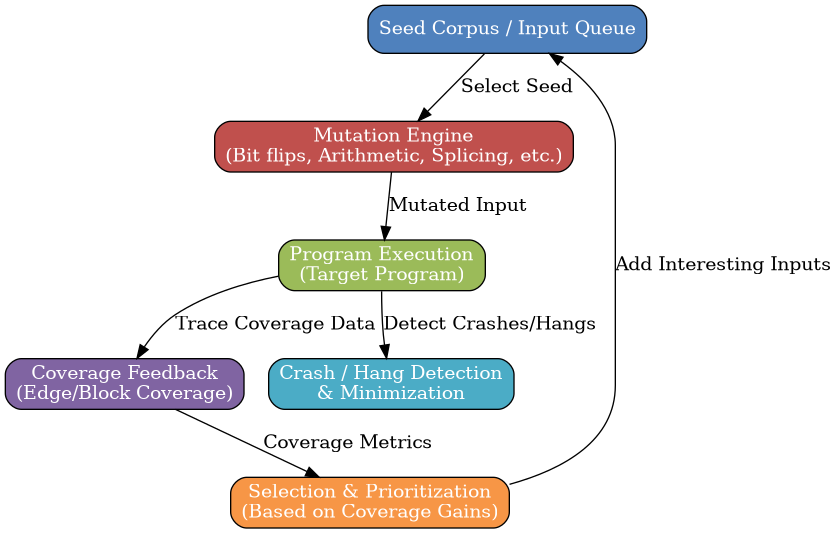
\includegraphics[width=.5\textwidth]{images/evo_fuzz.png} 
\end{frame}

\begin{frame}
\frametitle{Main Modules Description}
 
\begin{itemize}
    \item \textbf{Seed Corpus / Input Queue (Blue)}
    \begin{itemize}
        \item Holds the initial set of seed inputs and manages the queue of inputs waiting to be processed.
    \end{itemize}
    
    \item \textbf{Mutation Engine (Red)}
    \begin{itemize}
        \item Generates new test inputs by applying mutation strategies (e.g., bit flips, arithmetic operations, splicing).
    \end{itemize}
    
    \item \textbf{Program Execution (Green)}
    \begin{itemize}
        \item Executes the target program using mutated inputs, collects trace coverage data, and monitors for crashes or hangs.
    \end{itemize}
    
    \item \textbf{Crash / Hang Detection \& Minimization (Cyan)}
    \begin{itemize}
        \item Detects crashes or hangs during execution and minimizes the problematic inputs for debugging.
    \end{itemize}
    
    \item \textbf{Coverage Feedback (Purple)}
    \begin{itemize}
        \item Collects data on which parts of the program were exercised by the inputs to guide the fuzzing process.
    \end{itemize}
    
    \item \textbf{Selection \& Prioritization (Orange)}
    \begin{itemize}
        \item Selects and prioritizes inputs based on coverage metrics to discover new paths or trigger crashes.
    \end{itemize}
\end{itemize}
 
\end{frame}
 
\begin{frame}
\frametitle{Overall Flow}
 
\begin{enumerate}
    \item \textbf{Initialization}
    \begin{itemize}
        \item Start with a seed corpus or input queue containing initial test inputs.
    \end{itemize}
    
    \item \textbf{Mutation}
    \begin{itemize}
        \item Select seeds from the input queue and apply mutation strategies to generate new inputs.
    \end{itemize}
    
    \item \textbf{Execution}
    \begin{itemize}
        \item Execute the target program with mutated inputs, collect coverage data, and detect crashes or hangs.
    \end{itemize}
    
    \item \textbf{Detection and Minimization}
    \begin{itemize}
        \item Record detected crashes or hangs and minimize the inputs for debugging.
    \end{itemize}
    
    \item \textbf{Feedback and Prioritization}
    \begin{itemize}
        \item Use coverage feedback to evaluate inputs, select and prioritize those that improve coverage.
    \end{itemize}
    
    \item \textbf{Iteration}
    \begin{itemize}
        \item Iterate the process, refining inputs based on coverage feedback to maximize code exploration and crash discovery.
    \end{itemize}
\end{enumerate}
 
\end{frame}
\section{Case Study}
\begin{frame}{Background}
\begin{itemize}
\item Robotic software development exhibits stark contrasts to traditional software engineering paradigms
\item Simulators are a critical component of the software development toolchain for robotic systems
\item Gazebo has emerged as the \textit{de facto standard} for simulation in robotics
\item Applications: aerospace missions, subterranean exploration, maritime operational simulations
\end{itemize}
\end{frame}

\begin{frame}{Background: Challenges}
\begin{itemize}
\item Bugs in robotic simulators may result in:
  \begin{itemize}
  \item Simulation errors
  \item Data loss
  \item Vulnerability to malicious exploitation
  \item Compromised efficiency and quality of software development
  \end{itemize}
\item Testing robotic simulators like Gazebo is difficult due to:
  \begin{itemize}
  \item Strict Input Challenge
  \item State Space Challenge
  \end{itemize}
  \begin{figure}
  \begin{center}
      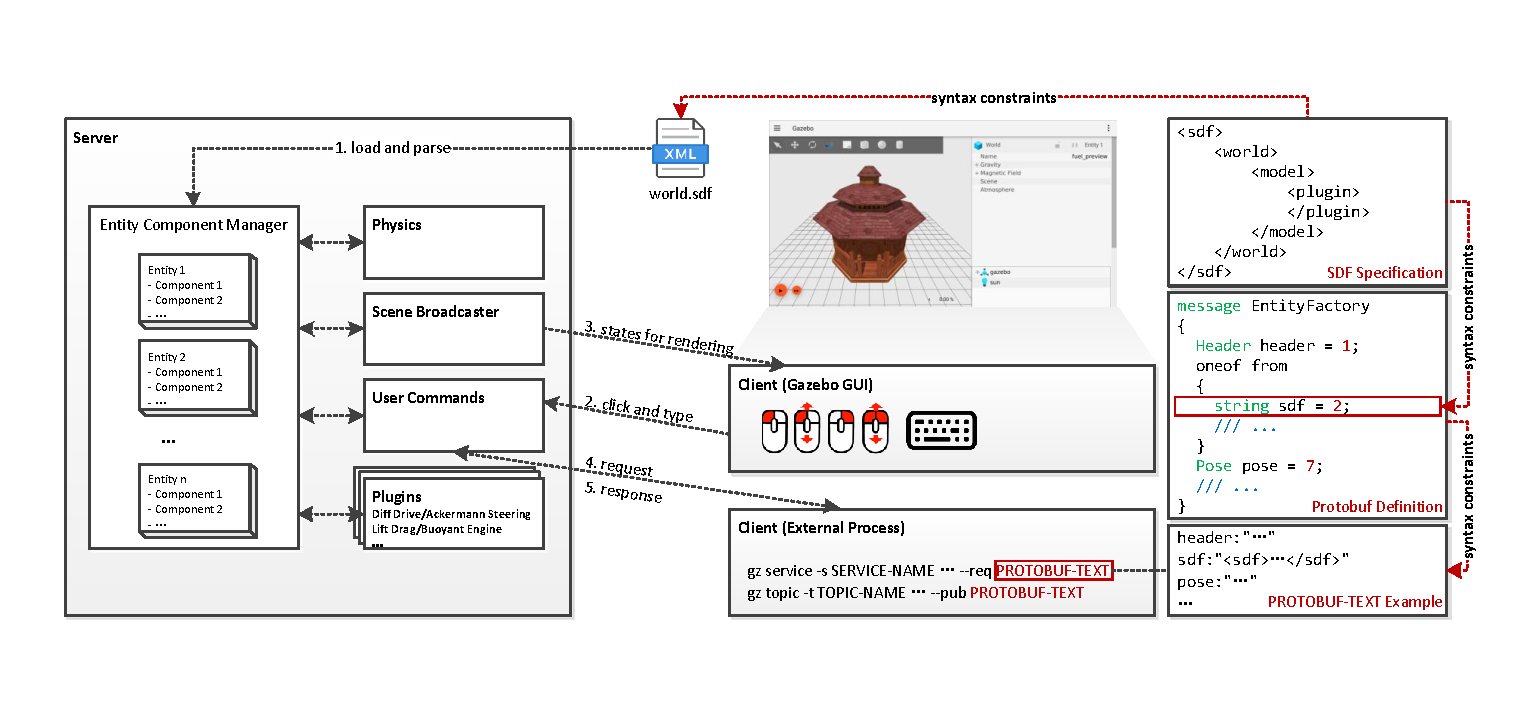
\includegraphics[width=.6\textwidth]{images/architecture.pdf}
  \end{center}
  \caption{Architecture of Gazebo}
  \label{fig:}
  \end{figure}
  
\end{itemize}
\end{frame}

\begin{frame}{Strict Input Challenge (Input File)}
\begin{center}
\includegraphics[width=0.8\textwidth]{example-image}
\end{center}
\begin{itemize}
\item SDF file $\rightarrow$ DOM tree $\rightarrow$ Rendered scenario
\item Load $\rightarrow$ Parse $\rightarrow$ Simulate
\end{itemize}
\end{frame}

\begin{frame}[fragile]{Strict Input Challenge (Command)}
\begin{verbatim}
gz service --timeout 10000 \
-s /world/default/create \
--reptype gz.msgs.Boolean \
--reqtype gz.msgs.EntityFactory \
--req 'sdf: "<model name=\"vehicle_blue\">...</model>"
pose {
  position {
    x: 2.3509603833593182
    y: 5.568459723740165
    z: 9.435891851259887
  }
}
name: "model"'
\end{verbatim}
\end{frame}

\begin{frame}{State Space Challenge}
\begin{itemize}
\item More than 100 plugins/modules
\item Joints/links/sensors dynamically created
\item More than 50 built-in services and topics
\item Plugin-specific services and topics
\item Command sequence of arbitrary length
\end{itemize}
\end{frame}

\begin{frame}[t]{Our Approach: GzFuzz}
\begin{itemize}
\item Syntax-aware Feasible Command Generation
\item Learning-based Command Generator Selection
\end{itemize}
\begin{center}
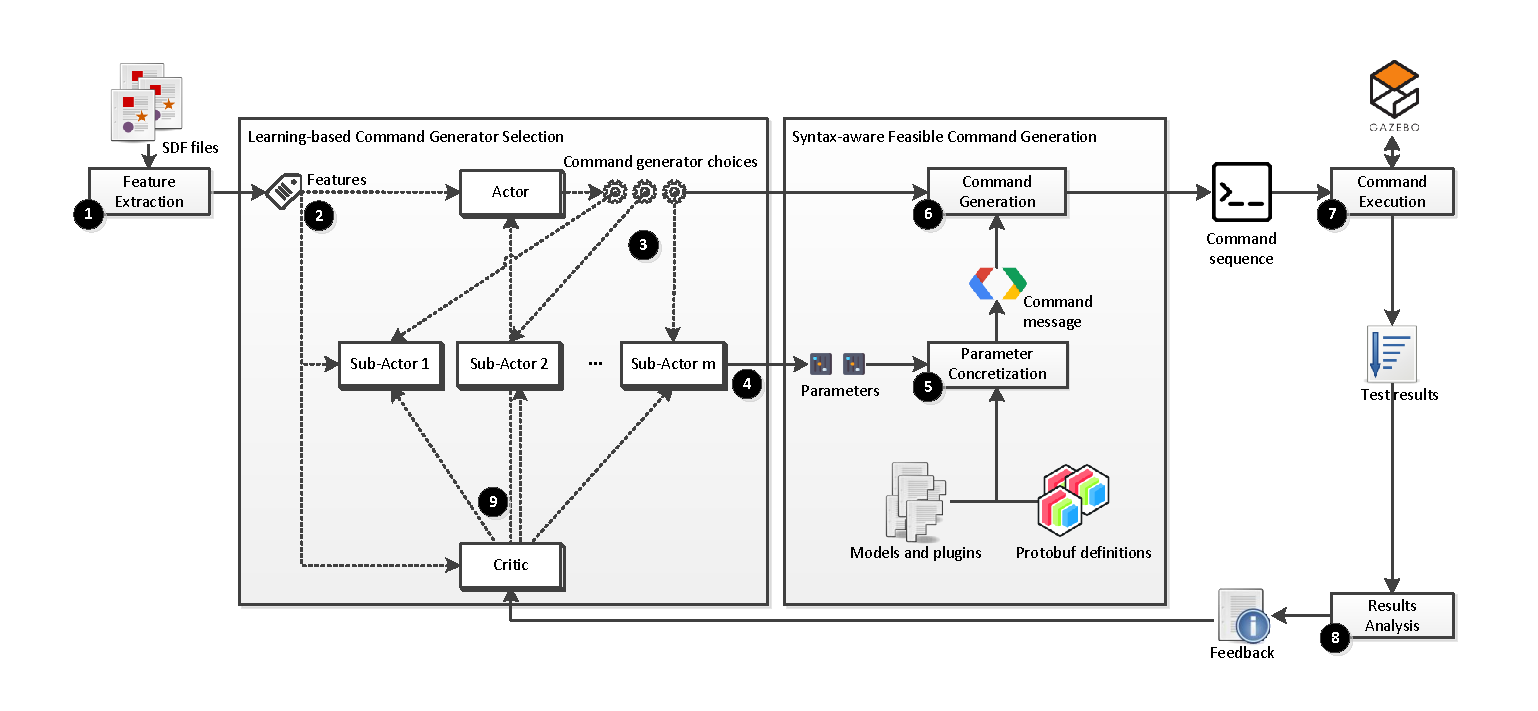
\includegraphics[width=0.9\textwidth]{images/workflow.pdf}
\end{center}
\end{frame}

\begin{frame}{Syntax-aware Feasible Command Generation}
\begin{itemize}
\item For Generators 6–9, further determine specific parameters
\item Ensures commands are both feasible and diverse
\end{itemize}
\end{frame}

\begin{frame}{Learning-based Command Generator Selection}
\begin{itemize}
\item Simplified hierarchical reinforcement learning (Advantage Actor-Critic)
\item Actors select command generators
\item Sub-Actors select parameters
\item Critic updates parameters of Actors and Sub-Actors
\item Reward based on crash, coverage improvement, and diversity
\end{itemize}
\end{frame}

\begin{frame}{Bug Detection}
\begin{itemize}
\item Commands executed with spawned Gazebo
\item Crash-based test oracle
\item Once crash detected:
  \begin{itemize}
  \item Command sequence iteratively reduced
  \item Manually checked
  \item Bug reports issued
  \end{itemize}
\end{itemize}
\end{frame}

\begin{frame}{Evaluation: Research Questions}
\begin{itemize}
\item \textbf{RQ1}: Is GzFuzz effective in finding bugs for Gazebo?
\item \textbf{RQ2}: How effective is GzFuzz compared with existing fuzzing methods?
\item \textbf{RQ3}: What is the impact of the two main components on GzFuzz?
\end{itemize}
\end{frame}

\begin{frame}{Evaluation Setup}
\begin{itemize}
\item Baselines: AFL++, Fuzzotron
\item Gazebo Version: latest dev (RQ1), Gazebo 8.0.0 (RQ2, RQ3)
\item Data: 309 SDF files, 123 modules with plugins, 117 plugins
\item Implementation: PyTorch, lxml, randomproto
\end{itemize}
\end{frame}

\begin{frame}{Evaluation Results}
\begin{center}
\includegraphics[width=0.8\textwidth]{example-image}
\end{center}
\end{frame}

\begin{frame}{Answer to RQ1}
\begin{itemize}
\item GzFuzz detected \textbf{25 unique crashes} in less than six months
\item \textbf{24 bugs} were fixed or confirmed
\end{itemize}
\end{frame}

\begin{frame}{Answer to RQ2}
\begin{itemize}
\item GzFuzz significantly outperforms baseline approaches
\item Over 12-hour testing: more bugs detected on previous Gazebo release
\item Statistically significant improvement
\end{itemize}
\end{frame}

\begin{frame}{Answer to RQ3}
\begin{itemize}
\item Syntax-aware generators and RL-based selection both contribute
\item Two mechanisms collectively enhance effectiveness
\end{itemize}
\end{frame}

\begin{frame}{Contributions}
\begin{itemize}
\item First study to apply fuzz testing to Gazebo
\item Syntax-aware feasible command generators
\item Learning-based command generator selection
\item 25 unique crashes detected, 24 fixed/confirmed
\end{itemize}
\end{frame}

\begin{frame}{Future Work}
\begin{itemize}
\item Incorporate differential testing across simulators
\item Integrate LLMs for more complex and realistic test cases
\end{itemize}
\end{frame}

\begin{frame}
\centering
\Large
Thank You\\
\vspace{1cm}
Zhilei Ren\\
\small
zren@dlut.edu.cn
\end{frame}

\end{document}

